% !TEX root = ../main.tex

\nop{
=========================================
Outline for Sec 4
\begin{itemize}
    \item First introduce how to tackle the problem (1) without considering the data privacy issue of all clients.
    \item asdf
\end{itemize}
}

\section{Federated Attentive Message Passing}
\label{sec:alg}
In this section, we first propose a general method to tackle the optimization problem in Eq.~\eqref{eq:our-form} without considering privacy preservation for clients.
Then, we implement the general method by a personalized federated learning method, \textit{federated attentive message passing} (FedAMP), which collaboratively trains the personalized models of all clients and preserves their data privacy.
Last, we explain why FedAMP can adaptively facilitate collaborations between clients and significantly improve the performance of the personalized models.

\nop{ iteratively encourage clients with similar model parameters to have much stronger collaboration than clients with dissimilar ones, such that, it can}

\nop{
Federated attentive message passing ({FedAMP}) is a general framework to tackle the personalized federated learning problem.
The \textbf{key idea} is to iteratively encourage clients with similar model parameters to have much stronger collaboration than clients with dissimilar ones, such that, we can adaptively discover the underlying collaboration relationships between clients, and further boosts their collaboration effectiveness.
}

\nop{Specifically, {FedAMP} promotes effective inter-client collaboration by realizing an \textbf{attentive collaboration mechanism} that iteratively encourages clients with more similar model parameters to have stronger collaborations.
}

\nop{that measures the similarity between model parameters in a non-linear manner with respect to their distance, and}

\nop{In this subsection, we first define the personalized federated learning problem, then we introduce how to tackle this problem by a general federated learning framework named federated attentive message passing ({FedAMP}).
}




\nop{
where $F_i:\R^d\rightarrow\R$ is the training objective function of the $i$-th client, $D(\cdot,\cdot)$ is a regularization function that measures the difference of its two inputs, and $\lambda>0$ is a regularization parameter. Roughly speaking, formulation Eq.~\eqref{eq:our-form} attempts to minimize the training loss of every personalized models $\{w_i\}_{i=1}^m$ and at the same time enforces collaboration by adding the regularization term. Formulations in a similar form of Eq.~\eqref{eq:our-form} have been adopted in multi-task learning (see, {\it e.g.}, \cite{han2015learning,zhang2017survey}).
}
\nop{
It is worth mentioning that formulations in a similar form of Eq.~\eqref{eq:our-form} have been adopted in multi-task learning (see, {\it e.g.}, \cite{han2015learning}) but most of the existing multi-task learning algorithms cannot tackle the common challenges of personalized federated learning, such as data privacy, communication efficiency, stragglers, and dropped clients~\cite{smith2017federated}. 
Besides, the {\sc Mocha} method recently proposed in \cite{smith2017federated} can be applied to Eq.~\eqref{eq:our-form} when $F_i$ is convex for all $i$. However, it cannot handle more challenging non-convex models such as deep neural network.
}

\nop{In order to promote attentive collaboration among the clients, we consider a class of regularization functions, named {\it attention-inducing functions}, that are defined as follows.}


\nop{
Specific examples of attntion-inducing function will be discussed later in Section \ref{sec:instances}.
}

\nop{
Functions that satisfy (i) and (ii) are abundant and we provide several examples later in Section \ref{sec:instances}.
}

\nop{applied to a class of problem Eq.~\eqref{eq:our-form} in which $D$ is any attention-inducing function that can be chosen by the user}

\nop{
We propose to tackle the problem formulated in Eq.~\eqref{eq:our-form} by a novel algorithm named {FedAMP}, which is powered by an incremental-type optimization method (\cite{bertsekas2011incremental}) and is carefully deployed on the client-sever system to fit the privacy-preserving requirement of personalized federated learning. 
}

\nop{
computes an intermediate variable $U^k$ by applying a gradient descent step to $\mD$, {\it i.e.},
}

\subsection{A General Method}
Denote by $\mF(W)\coloneqq\sum_{i=1}^m F_i(\mathbf{w_i})$ and $\mA(W)\coloneqq\sum_{i<j}^m A(\|\mathbf{w_i} - \mathbf{w_j}\|^2)$ the first and the second terms of $\mG(W)$, respectively. We can rewrite the optimization problem in Eq.~\eqref{eq:our-form} to
\begin{equation}
\label{eq:our-new-form}
\min_{W} \ \left\{\mG(W):= \mF(W) + \lambda \mA(W)\right\}.
\end{equation}

Based on the framework of incremental-type optimization~\cite{bertsekas2011incremental}, we develop a general method to iteratively optimize $\mG(W)$ by alternatively optimizing $\mA(W)$ and $\mF(W)$ until convergence.
In the $k$-th iteration, we first optimize $\mA(W)$  by applying a gradient descent step to compute an intermediate $d$-by-$m$ dimensional matrix
\begin{equation}
\label{eq:grad-descent-intro}
U^k = W^{k-1} - \alpha_k\nabla\mA(W^{k-1}),
\end{equation} 
where $\alpha_k>0$ is the step size of gradient descent, and $W^{k-1}$ denotes the matrix $W$ after the $(k-1)$-th iteration.
Then, we use $U^k$ as the prox-center and apply a proximal point step~\cite{rockafellar1976monotone} to optimize $\mF(W)$ by computing
\begin{equation}
\label{eq:ppa-intro}
W^k = \arg\min_{W} \ \mF(W) + \frac{\lambda}{2\alpha_k}\|W - U^k\|^2.
\end{equation}

This iterative process continues until a preset maximum number of iterations $K$ is reached.
As illustrated later in Section~\ref{sec:analysis}, we analyze the non-asymptotic convergence of the general method, and prove that it converges to an optimal solution when $\mG(W)$ is a convex function, and to a stationary point when $\mG(W)$ is non-convex.

\nop{
this general method non-asymptotically converges \chu{converges to what?} in both the situations when the function $\mG(W)$ is convex and non-convex, respectively.
}

\nop{
to the global optimum point when $\mG(W)$ is convex, and it converges to a local optimum point when $\mG(W)$ is non-convex.
}

\nop{
The non-asymptotic convergence guarantee of this general method is provided in Section~\ref{sec:analysis}.
}

\nop{
In order to conduct personalized federated learning, we regard 
}




\subsection{FedAMP}

The general method introduced above can be easily implemented by merging all clients' private training data together as the training data. To perform personalized federated learning without infringing the data privacy of the clients, we develop FedAMP to implement the optimization steps of the general method in a client-server framework by maintaining a personalized cloud model for each client on a cloud server, and passing weighted model-aggregation messages between personalized models and personalized cloud models.

\nop{
The \textbf{key idea} of FedAMP is to maintain a personalized cloud model for each client on a cloud server, and equivalently conduct the optimization steps of the general method by passing weighted model-aggregation messages between personalized models and personalized cloud models.
}

Following the optimization steps of the general method, FedAMP first optimizes $\mA(W)$ and implements the optimization step in Eq.~\eqref{eq:grad-descent-intro} by computing the $d$-by-$m$ dimensional matrix $U^k$ on the cloud server.

\nop{
Denote by $U^k=[u_1^k, \ldots, u_m^k]$, where the columns $u_1^k, \ldots, u_m^k$ are regarded as the model parameters of the personalized cloud models for each of the $m$ clients, respectively.
}
Let $U^k=[\mathbf{u_1^k}, \ldots, \mathbf{u_m^k}]$, where $\mathbf{u_1^k}, \ldots, \mathbf{u_m^k}$ are the $d$-dimensional columns of $U^k$.
Since $\mA(W):=\sum_{i<j}^m A(\|\mathbf{w_i} - \mathbf{w_j}\|^2)$ and $A(\|\mathbf{w_i} - \mathbf{w_j}\|^2)$ is an attention inducing function, the $i$-th column $\mathbf{u_i^k}$ of matrix $U^k$ computed in Eq.~\eqref{eq:grad-descent-intro} can be rewritten into a linear combination of the model parameter sets $\mathbf{w_1^{k-1}}, \ldots, \mathbf{w_m^{k-1}}$ as follows.
\begin{equation}
\begin{aligned}
\label{eq:grad-step-eq}
\mathbf{u_i^k} =& \left(1 - \alpha_k\sum_{j\neq i}^m A^\prime\left(\|\mathbf{w_i^{k-1}} - \mathbf{w_j^{k-1}}\|^2\right)\right)\cdot \mathbf{w_i^{k-1}} \\ 
&  + \alpha_k \sum_{j\neq i}^m A^\prime\left(\|\mathbf{w_i^{k-1}} - \mathbf{w_j^{k-1}}\|^2\right)\cdot \mathbf{w_j^{k-1}} \\
=& \xi_{i,1}\mathbf{w_1^{k-1}} + \dots + \xi_{i,m}\mathbf{w_m^{k-1}},
\end{aligned}
\end{equation}
where $A^\prime(\|\mathbf{w_i} - \mathbf{w_j}\|^2)$ is the derivative of $A(\|\mathbf{w_i} - \mathbf{w_j}\|^2)$ and $\xi_{i,1}, \ldots, \xi_{i,m}$ are the linear combination weights of the model parameter sets $\mathbf{w_1^{k-1}}, \ldots, \mathbf{w_m^{k-1}}$, respectively.



\nop{
and $\xi_{i,1} + \dots + \xi_{i,m} = 1$ always holds.
}

\nop{, and $u_i^k$ is the model parameters of the $i$-th client's personalized cloud model, that is, a convex combination of the messages received from all the clients including itself}

Often a small value is chosen as the step size $\alpha_k$ of gradient descent so that all the linear combination weights $\xi_{i,1}, \ldots, \xi_{i,m}$ are non-negative. Since $\xi_{i,1} + \cdots + \xi_{i,m} = 1$, $\mathbf{u_i^k}$ is actually a convex combination of the model parameter sets $\mathbf{w_1^{k-1}}, \ldots, \mathbf{w_m^{k-1}}$ of the personalized models of the clients.

\begin{figure}[t]
    \centering
    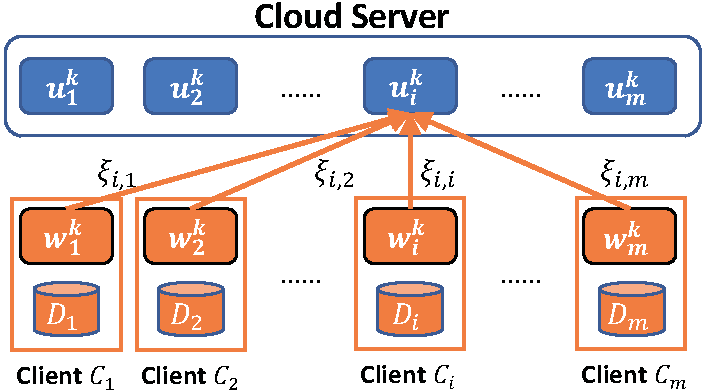
\includegraphics[width=0.36\textwidth]{figures/amp_mechanism.pdf} 
    \caption{The message passing mechanism of FedAMP.}
    \label{fig:mapmech}
\end{figure}

As illustrated in Figure~\ref{fig:mapmech}, the convex combination $\mathbf{u_i^k}$ can be modeled a \textit{message passing mechanism} as follows.
We treat $\mathbf{u_i^k}$ as the model parameter set of the \textit{personalized cloud model} of client $C_i$ and also a model aggregation that aggregates $\mathbf{w_1^{k-1}}, \ldots, \mathbf{w_m^{k-1}}$.
Correspondingly, we can treat $\mathbf{w_1^{k-1}}, \ldots, \mathbf{w_m^{k-1}}$ as \textit{model-aggregation messages} that are passed from all clients to client $C_i$ to conduct the model aggregation and produce $\mathbf{u_i^k}$ at the cloud server.


\nop{
we treat $\mathbf{u_i^k}$ as the model parameter sets of the \textit{personalized cloud model} $\mathcal{M}(\mathbf{u_i^k})$ \chu{owned by} the $i$-th client $C_i$, 

We also treat the parameter sets $\mathbf{w_1^{k-1}}, \ldots, \mathbf{w_m^{k-1}}$ as weighted \textit{model-aggregation messages} that are passed from each of the clients to client $C_i$ to conduct the model aggregation on the cloud server.
}

\nop{and
we regard $\mathbf{u_i^k}$ as the aggregation of the model parameter sets $\mathbf{w_1^{k-1}}, \ldots, \mathbf{w_m^{k-1}}$ of the personalized models owned by all clients. %\todo{Is $\mathbf{u_i^k}$ one number or a set of parameters?}
}

%\todo{What is $C_i$ here?  This paragraph is quite confusing.}

\nop{
by passing weighted model-aggregation messages between personalized models and personalized cloud models. 
}

The above message passing mechanism is the key step for FedAMP to perform inter-client collaboration.
This mechanism solely depends on the model parameter sets $\mathbf{w_1^{k-1}}, \ldots, \mathbf{w_m^{k-1}}$, thus the cloud server can collect $\mathbf{w_1^{k-1}}, \ldots, \mathbf{w_m^{k-1}}$ from the clients and conduct the message passing mechanism to optimize $\mA(W)$ without infringing the data privacy of all the clients.

\nop{
Moreover, 
}
After optimizing $\mA(W)$ on the cloud server, FedAMP then optimizes $\mF(W)$ and implements the optimization step in Eq.~\eqref{eq:ppa-intro} by computing independently columns $\mathbf{w_1^k}, \ldots, \mathbf{w_m^k}$ of $W^k$ for clients $C_1, \ldots, C_m$, respectively.
%
Recall that $\mathbf{w_i^k}$ is the model parameter set of the personalized model owned by client $C_i$. Following Eq.~\eqref{eq:ppa-intro}, we compute $\mathbf{w_i^k}$ locally on $C_i$ by 
\begin{equation}
\label{eq:local-training}
\mathbf{w_i^{k}} = \arg\min_{\mathbf{w}\in\R^d} F_i(\mathbf{w}) + \frac{\lambda}{2\alpha_{k}}\|\mathbf{w} - \mathbf{u_i^{k}}\|^2,
\end{equation}
Here, we only use the private training data set $D_i$ of client $C_i$ to perform personalized training on model $\mathcal{M}(\mathbf{w_i})$ and, at the same time, consider the inter-client collaboration information carried by the personalized cloud model $\mathcal{M}(\mathbf{u_i^k})$ by requiring $\mathbf{w_i^k}$ and $\mathbf{u_i^k}$ to be close to each other.


\nop{Say something here to clarify that (6) is doing personalization while considering the collaboration with the other clients.}

Since Eq.~\eqref{eq:local-training} only uses $F_i(\mathbf{w})$ and $\mathbf{u_i^k}$, where $F_i(\mathbf{w})$ is determined by the private training data $D_i$ of client $C_i$, $C_i$ can request its own model parameter set $\mathbf{u_i^k}$ from the cloud server and compute $\mathbf{w_i^k}$ locally without exposing its private training data $D_i$ to any other clients or the cloud server. 
%
Furthermore, since $\mathbf{u_i^k}$ is a convex combination of $\mathbf{w_1^k}, \ldots, \mathbf{w_m^k}$, a client $C_j$ cannot infer the personalized models of any other clients or the private data of any other clients.

\nop{
with $\beta_{k} = \alpha_k/\lambda$, where $\lambda$ is the regularization parameter in Eq.~\eqref{eq:our-form}.
}

\nop{
Following Eq.~\eqref{eq:ppa-intro}, the model parameter $w_i^k$ of the personalized model of client $C_i$ can be computed as
}





\nop{We will discuss why this message passing works in the end of this section.}


\nop{
\begin{equation}\label{eq:cloud-average}
u_i^k = \xi_{i,1}w_1^{k-1} + \dots + \xi_{i,m}w_m^{k-1},
\end{equation}
}




\nop{
$u_i^k\in \mathbb{R}^d$, $i\in\{1, \ldots, m\}$, is the $i$-th column of $U^k$.
}

Algorithm~\ref{alg:FedAMP} summarizes the pseudocode. 
FedAMP implements the optimization steps of the general method in a client-server framework, that is, iteratively optimizing $\mG(W)$ by alternatively optimizing $\mA(W)$ and $\mF(W)$ until a preset maximum number of iterations $K$ is reached.
The non-asymptotic convergence of FedAMP is exactly the same as the general method.
% due to the \chu{per-step equivalence} between the two methods. 
%chu{We prove this equivalence as follows.}
%\todo{The equivalence between the two methods needs to be proved.}

\nop{
\begin{thm}
\label{thm:equivalence}
FedAMP is equivalent to the general method.
\end{thm}

The proof of Theorem~\ref{thm:equivalence} is in \chu{Appendix~\ref{}.}

%The step 4 in Algorithm~\ref{alg:FedAMP} can be conducted in parallel because the computations on different clients are independent with each other. 
}

\subsection{Collaboration in FedAMP}



\nop{
while fitting the challenging privacy-preserving requirement. 
}
\nop{

Then, we compute the next iterate $W^k$ by applying a proximal point step \cite{rockafellar1976monotone} to $\mF$ with the intermediate variable $U^k$ being the prox-center, {\it i.e.},
}
% \nop{to meet the challenging requirements of personalized federated learning.
% }
% \nop{
% , such as data privacy, dirty data with noisy labels and dropped clients.
% }
% \nop{
% {FedAMP} is powered by an incremental type of optimization algorithm (see \cite{bertsekas2011incremental}) , and it is carefully deployed to meet the demand of federated learning environment. 
% }
% \nop{, that are stored on the server}

\nop{
\textbf{First}, the iteration of {FedAMP} starts with an initial guess of the model parameters, denoted by $(w_1^{0}, \dots, w_m^{0})$. These parameters are first obtained by separately pre-training the personalized models of each client using their local data, and then collected and stored on the server.

\textbf{Second}, at the $k$-th communication round, the server computes a set of personalized cloud models $(u_1^{k},\dots,u_m^{k})$ by Eq.~\eqref{eq:grad-descent-intro}.
}
% applying a gradient descent step on the regularization function $\mD(w_1,\dots,w_m):= \sum_{i<j}^mD(w_i,w_j)$ in Eq.~\eqref{eq:our-form}, {\it i.e.},
% \begin{equation}\label{eq:grad-step}
% u_i^{k} = w_i^{k-1} - \alpha_{k}\nabla_i\mD(w_1^{k-1},\dots,w_m^{k-1}), \quad  i=1,\dots,m,
% \end{equation}
% where $\alpha_{k}>0$ is the step size for the $k$-th communication round and $\nabla_i\mD$ stands for the partial gradient of $\mD$ with respect to $w_i$. 
\nop{
Since $\mD(W)=\sum_{i<j}^mD(w_i,w_j)$ and the function $D$ is an attention-inducing function in Definition \ref{defi:att-ind},
\eqref{eq:grad-descent-intro} can be equivalently written as
\begin{equation}
\begin{aligned}
\label{eq:grad-step-eq}
u_i^k = &\left(1 - \alpha_k\sum_{j\neq i}^m \mA^\prime\left(\|w_i^{k-1} - w_j^{k-1}\|^2\right)\right)\cdot w_i^{k-1} \\ 
& + \alpha_k \sum_{j\neq i}^m \mA^\prime\left(\|w_i^{k-1} - w_j^{k-1}\|^2\right)\cdot w_j^{k-1}
\end{aligned}
\end{equation}
for all $i\in\{1,\dots,m\}$, where $u_i^k$ is simply a weighted average of $(w_1^{k-1},\dots,w_m^{k-1})$. 
}

\nop{
\textbf{Third}, the server sends each personalized cloud model $u_i^{k}$ to client $i$ and requests it to perform local training with the knowledge of $u_i^{k}$.
Following Eq.~\eqref{eq:ppa-intro}, client $i$ computes an updated local model $w_i^{k}$ by
\nop{
\begin{equation}
\label{eq:local-training}
w_i^{k} = \arg\min_{w\in\R^d} F_i(w) + \frac{1}{2\beta_{k}}\|w - u_i^{k}\|^2
\end{equation}
}
with $\beta_{k} = \alpha_k/\lambda$, where $\lambda$ is the regularization parameter in Eq.~\eqref{eq:our-form}. 

\textbf{Last}, the server collects the updated local models $(w_1^{k},\dots,w_m^{k})$ and the system enters the $(k+1)$-th communication round. When {FedAMP} terminates at the $K$-th round for some user-specified $K$, each client $i$ holds a pair of $u_i^{K}$ and $w_i^{K}$, which can both be used for personalied inference tasks. 
% The whole procedure of {FedAMP} is summarized in Algorithm \ref{alg:FedAMP}. We establish the convergence guarantee of {FedAMP} in Section \ref{sec:analysis}.
}


\begin{algorithm}[t]
\DontPrintSemicolon
\SetKwInput{KwInput}{Input}               
\SetKwInput{KwOutput}{Output} 
\KwInput{$m$ clients, each holds a set of private training data and a personalized model to train.}
% , local training parameters $\{\beta_{k}\}\subset\R_{++}$}
\KwOutput{The trained model parameter sets $\mathbf{w_1^{K}},\dots, \mathbf{w_m^{K}}$ and $\mathbf{u_1^{K}},\dots, \mathbf{u_m^{K}}$.}

Randomly initialize $\mathbf{w_1^0}, \ldots, \mathbf{w_m^0}$ on the clients.

\For{$k=1,2,\dots,K$}{
Optimize $\mA(W)$: cloud server collects $\mathbf{w_1^{k-1}}, \ldots, \mathbf{w_m^{k-1}}$ from the clients to compute $\mathbf{u_1^{k}}, \dots, \mathbf{u_m^{k}}$ by Eq.~\eqref{eq:grad-step-eq}. \\

Optimize $\mF(W)$: each client $C_i$ requests $\mathbf{u_i^k}$ from the cloud server to compute $\mathbf{w_i^k}$ by Eq.~\eqref{eq:local-training}.
\nop{
\For{$i=1,2,\ldots,m$}{
    Client $C_i$ requests $u_i^k$ from the cloud server to compute $w_i^k$ by Eq.~\eqref{eq:local-training}.\\
}}
}
\caption{FedAMP}
\label{alg:FedAMP}
\end{algorithm}


\nop{
Now we discuss why FedAMP realizes the attentive collaboration between clients.
}

\nop{
\textbf{First of all}, since {FedAMP} never transfers the private data of any client, the data privacy of all clients is kept intact during the entire training process.
}

\nop{
\textbf{Second}, {FedAMP} is a message passing approach. We can observe from Eq.~\eqref{eq:grad-step-eq} that the cloud model $u^k_i$ can be rewritten in the following form
\begin{equation}\label{eq:cloud-average}
u_i^k = \xi_{i,1}w_1^{k-1} + \dots + \xi_{i,m}w_m^{k-1}
\end{equation}
where $\xi_{i,1} + \dots + \xi_{i,m} = 1$, and $(\xi_{i,1}, \ldots, \xi_{i,m})$ are linear combination weights for the client model parameters $(w_1^{k-1}, \ldots, w_m^{k-1})$.
Obviously, the client model parameters $(w_1^{k-1}, \ldots, w_m^{k-1})$ can be viewed as the \textbf{messages} that are \textbf{passed} from all clients to the $i$-th client, and the model parameters $u_i^k$ of client $i$'s personalized cloud model is a weighted aggregation of the messages received from all clients.
As a result, {FedAMP} is a message passing approach that conducts inter-client collaboration by passing messages between local models and personalized cloud models. 
}

\nop{===============}

FedAMP adaptively facilitates collaborations between similar clients, since the attentive message passing mechanism iteratively encourages similar clients to collaborate more with each other during the personalized federated learning process.


\nop{
why the message passing process in Eq.~\eqref{eq:grad-step-eq} is attentive, that is, it encourages similar clients to collaborate more with each other, and further conclude the potential of this attentive message passing process in adaptively discovering the underlying collaboration relationships between clients.
}

To analyze the attentive message passing mechanism of FedAMP, 
we revisit the weights $\xi_{i,1}, \ldots, \xi_{i,m}$ of the convex combination in Eq.~\eqref{eq:grad-step-eq}, where the weight
\begin{equation}
\label{eq:attentive-mechanism}
    \xi_{i,j}=\alpha_k A^\prime\left(\|\mathbf{w_i^{k-1}} - \mathbf{w_j^{k-1}}\|^2\right), (i\neq j)
\end{equation}
is the contribution of message $\mathbf{w_j^{k-1}}$ sent from client $C_j$ to the aggregated model parameter set $\mathbf{u_i^{k}}$ of the personalized cloud model owned by client $C_i$.
$\xi_{i,i} = 1 - \sum_{j\neq i}^m \xi_{i,j}$
is simply a self-attention weight that specifies the proportion of the model parameter set $\mathbf{w_i^{k-1}}$ of client $C_i$'s personalized model in its own personalized cloud model.

Due to Definition \ref{defi:att-ind}, $A$ is an increasing and concave function on $[0,\infty)$. Thus, the derivative $A^\prime$ of $A$ is a non-negative and non-increasing function on $(0,\infty)$.
Therefore, function $A^\prime(\|\mathbf{w_i^{k-1}} - \mathbf{w_j^{k-1}}\|^2)$ is a \textit{similarity function} that measures the similarity between $\mathbf{w_i^{k-1}}$ and $\mathbf{w_j^{k-1}}$, such that their similarity is high if they have a small Euclidean distance.

From Eq.~\eqref{eq:attentive-mechanism},
if the model parameters $\mathbf{w_i^{k-1}}$ and $\mathbf{w_j^{k-1}}$ are similar with each other, they contribute more to the model parameters $\mathbf{u_j^k}$ and $\mathbf{u_i^k}$ of clients $C_j$ and $C_i$, respectively.
This further makes $\mathbf{u_i^k}$ and $\mathbf{u_j^k}$ more similar to each other.
Since the optimization step in Eq.~\eqref{eq:local-training} forces $\mathbf{w_i^k}$ and $\mathbf{w_j^k}$ to be close to $\mathbf{u_i^k}$ and $\mathbf{u_j^k}$, respectively, $\mathbf{w_i^k}$ and $\mathbf{w_j^k}$ are more similar to each other as well.
 
In summary, FedAMP builds a positive feedback loop that iteratively encourages clients with similar model parameters to have stronger collaborations, and adaptively and implicitly groups similar clients together to conduct more effective collaborations.
%This is exactly how FedAMP discovers the underlying collaboration relationships between similar clients. 
%As demonstrated later in Section~\ref{sec:exp}, FedAMP accurately discovers the group collaboration structure of clients and achieves outstanding personalized federated learning performance.

\nop{
a message $w_j^{k-1}$ that is similar to $w_i^{k-1}$ contributes more to the model parameters $u_i^k$ of the personalized cloud model owned by client $C_i$.
This in-turn makes $u_i^k$ to be more similar to $w_j^{k-1}$ as well.
}

\nop{
Since the optimization step in Eq.~\eqref{eq:local-training} forces $w_i^k$ to be close to $u_i^k$, $w_i^k$ should also be close to $w_j^{k-1}$ as well.

In this way, FedAMP iteratively encourages clients with more similar model parameters to have stronger collaborations, which makes it possible to adaptively discover the underlying collaboration relationships between similar clients.
}

\nop{
As a result, {FedAMP} realizes the attentive collaboration mechanism.
}

\nop{
When $i=j$, the weight $\xi_{i,i}$ of the message $w_i^{k-1}$ passed from client $C_i$ to its own personalized cloud model is
\begin{equation}\nonumber
    \xi_{i,i}=1 - \sum_{j\neq i}^m \xi_{i,j}.
\end{equation}

}


\nop{
as
\begin{equation}\nonumber
%\label{eq:grad-step-cvx-combi}
u_i^k = \tau_{k,i}w_i^{k-1} + (1-\tau_{k,i})z_i^{k-1},
\end{equation}
where 
\begin{equation} 
\label{eq:colla-center}
z_i^{k-1} = \frac{\sum_{j\neq i}^m \mA^\prime(\|w_i^{k-1} - w_j^{k-1}\|^2)\cdot w_j^{k-1}}{\sum_{j\neq i}^m \mA^\prime(\|w_i^{k-1} - w_j^{k-1}\|^2)},
\end{equation}
is an aggregation of the messages from all the clients other than client $i$, and 
\begin{equation}\nonumber
\tau_{k,i} = 1 - \alpha_k\sum_{j\neq i}^m \mA^\prime(\|w_i^{k-1} - w_j^{k-1}\|^2)
\end{equation}
is a scalar self-attention parameter that balances the contribution of the messages received by $u_i^k$ from client $i$ and the other clients.

Recall Definition \ref{defi:att-ind} that $\mA$ is increasing and concave on $[0,\infty)$, which implies that its derivative $\mA^\prime$ is non-negative and non-increasing on $(0,\infty)$. Thus, the $z_i^{k-1}$ in Eq.~\eqref{eq:colla-center} is a convex combination of $\{w_j^{k-1}: j\neq i\}$. 
Since the weight of each $w_j^{k-1}$ in Eq.~\eqref{eq:colla-center} is non-negative and its magnitude is a non-increasing function of the Euclidean distance between $w_j^{k-1}$ and $w_i^{k-1}$, a $w_j^{k-1}$ that is similar to $w_i^{k-1}$ contributes more to the aggregation Eq.~\eqref{eq:colla-center}. 
In this way, {FedAMP} iteratively encourages clients with more similar model parameters to have stronger collaborations. As a result, {FedAMP} realizes the attentive collaboration mechanism.
}

\nop{
In summary, FedAMP realizes the optimization steps of the general method by passing weighted model aggregation messages between personalized models and personalized cloud models.
This allows each client to collaboratively train its own personalized model without infringing the data privacy of the other clients.
}

\nop{
It is worth mentioning that the mechanism of collaboration in {FedAMP} is blind to the clients. This means each client receives a tailored cloud model $u_i^k$ without knowing the collaboration graph, which further improves the privacy of all clients during training.
}

\nop{
It is worth mentioning that, with the flexibility of choosing the function $\mA$, we can control the degree of non-linearity of the attentive collaboration mechanism, which has been documented to be significant in many applications (see, {\it e.g.}, \cite{sabour2017dynamic}). 
Moreover, the attention-inducing function $D$ is the choice of the server, thus the mechanism of collaboration in {FedAMP} is blind to the clients. This means each client receives a tailored cloud model $u_i^k$ without knowing the collaboration graph, which further improves the privacy of all clients during training.
}
\nop{
Next, we discuss how {FedAMP} tackles the aforementioned personalization and privacy challenges in personalized federated learning. First, {FedAMP} allows each client $i$ to hold a \emph{personalized local model} $w_i^k$ and trains these models without infringing the data privacy of each client. These models are the only messages passed from each client to the server for collaboration. Second, in contrast with many existing methods such as FedAvg and FedProx, where a single cloud model ({\it i.e.}, the global model) is sent to all the clients, {FedAMP} allows the server to provide \emph{personalized guidance} to each client $i$ through a cloud model $u_i^k$ that is tailored for client $i$. In particular, observe from Eq.~\eqref{eq:grad-step-eq} that the cloud model $u^k_i$ is of the form
\begin{equation}\label{eq:cloud-average}
u_i^k = \xi_{i,1}w_1^{k-1} + \dots + \xi_{i,m}w_m^{k-1}
\end{equation}
with $\xi_{i,1} + \dots + \xi_{i,m} = 1$. Here, the aggregation weights $\{\xi_{i,j}\}_{j=1}^m$ in Eq.~\eqref{eq:cloud-average} are tailored for client $i$ and different clients may have distinct weight parameters. 
% This contrasts with existing methods such as FedAvg and FedProx, where the server provides identical guidance to all the clients via a single cloud model, or equivalently, the $\xi_{i,j}$ in Eq.~\eqref{eq:cloud-average} is constant for all $i$. 


Next, we discuss how {FedAMP} invokes attentive collaboration among the clients. With the $D$ in Eq.~\eqref{eq:our-form} being an attention-inducing function, the personalized cloud models $u_i^k$ for every client $i$ are constructed in an attentive manner. To see this, we rewrite Eq.~\eqref{eq:grad-step-eq} as
\begin{equation}
\label{eq:grad-step-cvx-combi}
u_i^k = \tau_{k,i}w_i^{k-1} + (1-\tau_{k,i})z_i^{k-1},
\end{equation}
where $\tau_{k,i} = 1 - \alpha_k\sum_{j\neq i}^m \mA^\prime(\|w_i^{k-1} - w_j^{k-1}\|^2)$ is a scalar self-attention parameter that balances the contribution of the message from client $i$ itself and the messages passed from clients other than $i$ to $u_i^k$, and $z_i^{k-1}$ is an aggregation of the messages from all the clients other than $i$:
\begin{equation}
\label{eq:colla-center}
z_i^{k-1} = \frac{\sum_{j\neq i}^m \mA^\prime(\|w_i^{k-1} - w_j^{k-1}\|^2)\cdot w_j^{k-1}}{\sum_{j\neq i}^m \mA^\prime(\|w_i^{k-1} - w_j^{k-1}\|^2)}.
\end{equation}
Recall from Definition \ref{defi:att-ind} that $\mA$ is increasing and concave on $[0,\infty)$, which implies that its derivative $\mA^\prime$ is non-negative and non-increasing on $(0,\infty)$. Thus, the $z_i^{k-1}$ in Eq.~\eqref{eq:colla-center} is a convex combination of $\{w_j^{k-1}: j\neq i\}$ with an attentive mechanism. Indeed, the weight of each $w_j^{k-1}$ in Eq.~\eqref{eq:colla-center} is non-negative and its magnitude is a non-increasing function of the Euclidean distance between $w_j^{k-1}$ and $w_i^{k-1}$, indicating that an $w_j^{k-1}$ that is similar to $w_i^{k-1}$ contributes more to the aggregation Eq.~\eqref{eq:colla-center}. Moreover, with the flexibility of choosing the function $\mA$, we can control the degree of non-linearity of the attentive mechanism, which has been documented to be significant in many applications (see, {\it e.g.}, \cite{sabour2017dynamic}). Finally, we remark that the attention-inducing function $D$ is the choice of the server and thus the mechanism of collaboration in {FedAMP} is blind to the clients. In particular, each client receives a tailored cloud model $u_i^k$ without knowing the collaboration graph. 
}

\nop{
As illustrated later in Section~\ref{sec:instances}, a properly designed function $D$ produces the attentive message passing (AMP) mechanism that encourages closely related clients to collaborate more during training.
This allows {FedAMP} to adaptively discover the underlying collaboration relationships between clients without infringing their data privacy, which significantly boosts the effectiveness of client collaborations and leads to the outstanding performance of {FedAMP}.
d, for example, by separately pre-training on each client with their local data and then collected by the server.

\textbf{Second}, as we shall elaborate in Section \ref{sec:instances}, for many attention-inducing functions $D$ in Eq.~\eqref{eq:our-form}, the gradient descent step in Eq.~\eqref{eq:grad-step} amounts to attentively aggregating the models. In particular, for every $i$, the personalized cloud model $u_i^{k}$ can be written as a convex combination of $(w_1^{k},\dots,w_m^{k})$, {\it i.e.}, 
%$u_i^{k} = \xi_{1}w_1^{k} + \dots + \xi_{m}w_m^{k}$
\begin{equation}
\label{eq:weight-average}
u_i^{k} = \xi_{i1}w_1^{k} + \dots + \xi_{im}w_m^{k},
\end{equation}
where aggregation weights $\xi_{ij} \geq 0$ and $\sum_{j=1}^m \xi_{ij} = 1$. Moreover, the magnitude of $\xi_{ij}$ is proportional to the distance between $w_i^{k}$ and $w_j^{k}$, leading to an attentive mechanism in aggregation Eq.~\eqref{eq:weight-average}. Furthermore, the mechanism in aggregation is blind to the clients, as the attention-inducing function $D$ is chosen by the server and does not need to be shared with the clients.

\textbf{Last}, one can observe that we require an exact computation in Eq.~\eqref{eq:grad-step} but allow an approximate solution in Eq.~\eqref{eq:local-training}. This is due to the fact that the computation in Eq.~\eqref{eq:grad-step} is performed on the server, which is stable and can be well controlled, while the computation in Eq.~\eqref{eq:local-training} is performed across the heterogeneous networks, where stragglers or even dropped clients are common. Details on the approximation criterion for Eq.~\eqref{eq:local-training} shall be specified in Section \ref{sec:analysis} when we analyze the convergence of the {FedAMP} framework. In practice, one may simply apply a number of epochs of stochastic optimization algorithms to obtain an updated model $w_i^{k}$ in Eq.~\eqref{eq:local-training}. 
}

\nop{
\begin{itemize}
\item[(i)] The initial models $(w_1^{0}, \dots, w_m^{0})$ can be obtained, for example, by separately pre-training on each client with their local data and then collected by the server.

\item[(ii)] As we shall elaborate in Section \ref{sec:instances}, for many distance-like functions $D$ in Eq.~\eqref{eq:our-form}, the gradient descent step in Eq.~\eqref{eq:grad-step} amounts to attentively aggregating the models. In particular, for every $i$, the personalized cloud model $u_i^{k}$ can be written as a convex combination of $(w_1^{k},\dots,w_m^{k})$, {\it i.e.}, 
%$u_i^{k} = \xi_{1}w_1^{k} + \dots + \xi_{m}w_m^{k}$
\begin{equation}
\label{eq:weight-average}
u_i^{k} = \xi_{1}w_1^{k} + \dots + \xi_{m}w_m^{k}
\end{equation}
for some non-negative weights $\{\xi_{j}\}_{j=1}^m$ such that $\xi_1 + \dots + \xi_m = 1$. Moreover, the magnitude of $\xi_j$ is proportional to the similarity between $w_i^{k}$ and $w_j^{k}$, leading to an attentive mechanism in aggregation Eq.~\eqref{eq:weight-average}. Furthermore, the mechanism in aggregation is blind to the clients, as the distance-like function $D$ is chosen by the server and does not need to be shared with the clients.

\item[(iii)] One can observe that we require an exact computation in Eq.~\eqref{eq:grad-step} but allow an approximate solution in Eq.~\eqref{eq:local-training}. This is due to the fact that the computation in Eq.~\eqref{eq:grad-step} is performed on the server, which is stable and can be well controlled, while the computation in Eq.~\eqref{eq:local-training} is performed across the heterogeneous networks, where stragglers or even dropped clients are common. Details on the approximation criterion for Eq.~\eqref{eq:local-training} shall be specified in Section \ref{sec:analysis} when we analyze the convergence of the FedAMP framework. In practice, one may simply apply a number of epochs of stochastic optimization algorithms to obtain an updated model $w_i^{k}$ in Eq.~\eqref{eq:local-training}. 
\end{itemize} 
}
%
%
%
%\begin{align}
%    D(x,y) & = \frac{1}{2}\|x - y\|^2, \label{eq:ec-dist} \\
%    D(x,y) & = \|x - y\|, \label{eq:norm-dist} \\
%    D(x,y) & = 1 - e^{-\frac{\|x - y\|^2}{2\sigma}}, \label{eq:Gauss-dist}
%\end{align}